% !TeX program = pdflatex
% Research Proposal -- 1501830 Topics in Artificial Intelligence (IEEE conference style)
\documentclass[conference]{IEEEtran}
\usepackage{cite}
\usepackage{iftex}
\ifXeTeX % local Tectonic build: use Times like IEEEtran does under pdfLaTeX
  \usepackage{fontspec}\setmainfont{texgyretermes}[Extension=.otf,UprightFont=*-regular,BoldFont=*-bold,ItalicFont=*-italic,BoldItalicFont=*-bolditalic]
\fi
\usepackage{amsmath,amssymb}
\usepackage{graphicx}
\usepackage{xcolor}
\usepackage{booktabs}
\usepackage{array}
\newcolumntype{L}[1]{>{\raggedright\arraybackslash}p{#1}}
\usepackage{tikz}
\usetikzlibrary{positioning,arrows.meta}
\usepackage{url}
\usepackage{balance}
\newcommand{\todo}[1]{{\color{red}[#1]}}
\newif\ifsurvey \surveyfalse % set \surveytrue only for an approved systematic-review project

\begin{document}

\title{CODA: Reliable False-Alarm Control for Quantized Anomaly Detectors on Heterogeneous Microcontrollers}

\author{\IEEEauthorblockN{Abdelaziz Saud}
\IEEEauthorblockA{PhD Program: Computer Science\\
University of Sharjah\\
Student ID: U25200513 \quad Email: U25200513@sharjah.ac.ae\\
Course 1501830, Fall 2026/2027 \quad Instructor: Dr.\ Hamza Ouarnoughi}}

\maketitle

\begin{abstract}
Anomaly detectors for cyber-physical systems are calibrated at full precision and then quantized to run on microcontrollers. Quantization shifts the anomaly-score distribution while largely preserving its ranking, so a conformal threshold inherited from the full-precision model can lose its false-alarm guarantee while accuracy metrics such as AUC show no change. We propose CODA (Calibrate Once, Deploy Anywhere), which calibrates the threshold once on a host GPU and gives each device a label-free correction measured from how its integer arithmetic perturbs the score. We will test whether this keeps the realized false-alarm rate within a target bound on three microcontroller families (STM32, ESP32, RP2350) using public industrial anomaly-detection benchmarks, and report latency and memory overhead on each board.
\end{abstract}

\begin{IEEEkeywords}
conformal prediction, anomaly detection, quantization, TinyML, cyber-physical systems
\end{IEEEkeywords}

\section{Problem Statement and Motivation}
Industrial sensors increasingly detect faults on the device itself, which cuts latency and keeps raw data local. To fit in kilobytes of SRAM, models are converted to 8-bit integers (INT8) after training~\cite{jacob2018,david2021,lin2020}. Operators also need a predictable false-alarm rate. Conformal anomaly detection sets a threshold that bounds false alarms on normal data at a chosen level $\alpha$~\cite{bates2023,angelopoulos2023}. This bound holds only for the model used in calibration.

In practice, the threshold is set once at full precision and copied to every device. Each device runs a different integer model, with its own kernels and rounding, so its scores drift and the guarantee is lost. Recalibrating each device is often impractical. The calibration set may not fit in flash, and its owner may not be allowed to copy it to every device in a fleet.

\textbf{Research question:} Can a threshold calibrated once at full precision, plus a label-free per-device shift correction, keep the realized false-alarm rate of INT8 anomaly detectors on heterogeneous microcontrollers within a target bound?\\
\textbf{Hypothesis:} On all three boards, the corrected threshold keeps the false-alarm rate on normal test data within $\alpha+\delta$ (with $\delta=0.01$, for $\alpha\in\{0.01,0.05\}$), while the inherited threshold exceeds it, and detection recall stays within 5 percentage points of per-device recalibration.

\begin{figure*}[t]
\centering
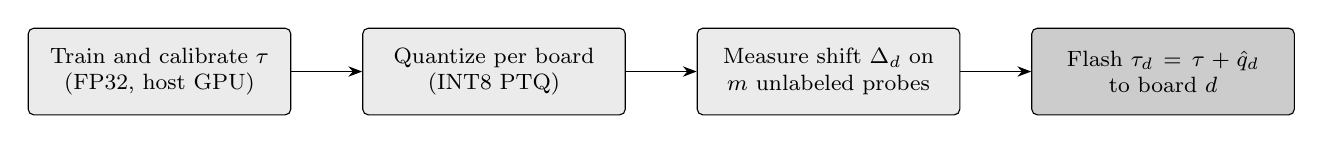
\begin{tikzpicture}[node distance=0.9cm, box/.style={draw, rounded corners=2pt, fill=black!8, align=center, font=\footnotesize, minimum height=1.1cm, text width=3.1cm}, >={Stealth[length=5pt]}]
\node[box] (a) {Train and calibrate $\tau$\\ (FP32, host GPU)};
\node[box, right=of a] (b) {Quantize per board\\ (INT8 PTQ)};
\node[box, right=of b] (c) {Measure shift $\Delta_d$ on\\ $m$ unlabeled probes};
\node[box, right=of c, fill=black!20] (d) {Flash $\tau_d=\tau+\hat q_d$\\ to board $d$};
\draw[->] (a) -- (b); \draw[->] (b) -- (c); \draw[->] (c) -- (d);
\end{tikzpicture}
\caption{The CODA pipeline. Calibration data stays on the host; each board receives one number, $\tau_d$.}
\label{fig:pipeline}
\end{figure*}

\section{Related Work and Research Gap}
Table~\ref{tab:rw} summarizes the closest work. A NeurIPS 2026 workshop study showed that 4-bit quantization of robot-policy failure detectors leaves AUC almost unchanged while the coverage of an inherited conformal threshold drops from 0.77 to 0.41 (target 0.90), because quantization roughly translates the score distribution~\cite{vla2026}; its repair is empirical and its quantization simulated. A 2026 benchmark measured conformal prediction on compressed LLMs, but recalibrates every compressed model~\cite{compress2026}. A retrieval study gives a conformal certificate that quantized and full-precision outputs agree~\cite{retrieval2026}; it does not address false alarms. On microcontrollers, TCUQ and HDUQ-HAR run conformal calibration on the deployed model directly~\cite{tcuq2025,hduq2026}. INT8 kernel paths on different hardware also diverge layer by layer~\cite{alibi2026}, which suggests that each chip needs its own correction. Conformal theory for non-exchangeable data exists~\cite{barber2023,gibbs2021} but has not been applied to this setting.

\begin{table}[t]
\caption{Closest work and what it leaves open}
\label{tab:rw}
\centering\footnotesize
\begin{tabular}{@{}L{2.0cm}L{2.9cm}L{2.9cm}@{}}
\toprule
Work & Contribution & Open\\ \midrule
VLA monitors~\cite{vla2026} & Inherited threshold fails under quantization & No guarantee; simulated; not sensors\\
LLM benchmark~\cite{compress2026} & Conformal on compressed LLMs & Recalibrates each model\\
Retrieval~\cite{retrieval2026} & Certifies FP/INT agreement & Not false-alarm control\\
TCUQ, HDUQ~\cite{tcuq2025,hduq2026} & On-MCU conformal & No FP-to-INT transfer\\
\bottomrule
\end{tabular}
\end{table}

To our knowledge, no existing method restores a conformal false-alarm guarantee for a full-precision threshold deployed on integer hardware, with proof, on real microcontrollers, for streaming sensor data.

\section{Proposed Method}
\subsection{Problem Formulation}
Let $x$ be a sensor window, $s(x)$ the full-precision anomaly score, and $s_d(x)$ the score of the INT8 model on device $d$. Split-conformal calibration on $n$ normal windows sets $\tau$ as the $\lceil (n+1)(1-\alpha)\rceil$-th smallest calibration score~\cite{bates2023}. With score shift $\Delta_d(x)=s_d(x)-s(x)$, we set
\begin{equation}
\tau_d=\tau+\hat q_d,
\end{equation}
where $\hat q_d$ is the $\lceil (m+1)(1-\delta)\rceil$-th smallest of $\Delta_d$ over $m$ unlabeled probe windows. A union bound gives a false-alarm rate on device $d$ of at most $\alpha+\delta$ when probe and test windows are exchangeable; we will prove this formally and extend it to temporally dependent data using block calibration~\cite{barber2023}.

\subsection{Approach}
Fig.~\ref{fig:pipeline} shows the pipeline. (1) Windows of length 64 (stride 1) are z-normalized with training statistics. (2) A 1D-convolutional autoencoder (three conv layers, under 100\,KB in INT8) is trained on normal windows; the score is reconstruction mean-squared error. The last 20\% of normal training data, split in time, is the calibration set. (3) Each board's model is produced by TensorFlow Lite full-integer post-training quantization with 500 representative windows, and compiled with TFLite Micro using CMSIS-NN (STM32, RP2350) or ESP-NN (ESP32)~\cite{david2021}. (4) $m=500$ probe windows are streamed to each board over UART; on-device scores give $\Delta_d$. (5) $\tau_d$ is flashed to the board. No calibration data leaves the host.


\section{Evaluation Plan}
\subsection{Datasets and Baselines}
The primary benchmark is the Server Machine Dataset (SMD)~\cite{su2019}. SWaT (water treatment, available on request) is the industrial case, and NASA SMAP/MSL is the backup. Common anomaly benchmarks have known labeling flaws~\cite{wu2023}, so the main metric is the false-alarm rate on normal data, where labels are least disputed.

The boards are an STM32 Nucleo (Cortex-M4/M7), an ESP32-S3 (Xtensa LX7), and a Raspberry Pi Pico~2 (RP2350, Cortex-M33), costing under 100~USD in total. Training uses existing lab GPUs.

We compare against four baselines: (B1) the inherited threshold $\tau$; (B2) per-device recalibration with the full calibration set, as an upper bound; (B3) on-device streaming quantile recalibration, following TCUQ and adaptive conformal inference~\cite{tcuq2025,gibbs2021}; and (B4) the label-free realignment repair of~\cite{vla2026}.

\subsection{Metrics}
Task metrics: realized false-alarm rate versus target $\alpha\in\{0.01,0.05,0.1\}$, detection recall, and AUC. Systems measures: inference latency per window (on-chip cycle counter), peak SRAM, and flash, including the overhead of the correction. All results are averaged over 5 seeds (training and calibration split), with 95\% confidence intervals.

\subsection{Ablations and Comparisons}
Table~\ref{tab:exp} lists the planned experiments. E1 tests the failure; E2 tests the hypothesis against B1--B4; E3 and E4 are ablations on probe source and size, and on bit-width and model size.

\begin{table}[t]
\caption{Planned experiments}
\label{tab:exp}
\centering\footnotesize
\begin{tabular}{@{}lL{2.2cm}L{2.3cm}L{2.0cm}@{}}
\toprule
ID & Question & Variants & Output\\ \midrule
E1 & Does inheriting $\tau$ break? & 3 boards, 3 datasets & FAR vs.\ $\alpha$, AUC\\
E2 & Does $\tau_d$ hold? & Ours vs.\ B1--B4 & FAR, recall, latency, SRAM\\
E3 & Is the shift numerical? & Probes: in-domain, other dataset, synthetic; $m\in\{50,200,500\}$ & FAR vs.\ probe source, $m$\\
E4 & Robust to compression? & INT8 vs.\ INT4; 3 model sizes & FAR, recall, memory\\
\bottomrule
\end{tabular}
\end{table}

\section{Risk Analysis}
The largest risk is that the score shift depends on the input data and not only on the integer arithmetic. In that case a generic probe set would give the wrong correction; experiment E3 tests this directly. Table~\ref{tab:risk} lists all risks with their mitigations.

\begin{table}[t]
\caption{Risk register}
\label{tab:risk}
\centering\footnotesize
\begin{tabular}{@{}L{2.3cm}L{0.75cm}L{4.65cm}@{}}
\toprule
Risk & Level & Mitigation\\ \midrule
Technical: shift depends on data (H2 fails) & M & Keep a small in-domain probe set on the host; report how much is needed\\
Technical: bound too loose & M & Tighter joint quantile instead of union bound\\
Novelty: ``why not recalibrate per device?'' & M & Quantify data size, privacy, and fleet cost; report B2 as upper bound\\
Data: SWaT access delayed & M & Start with SMD and SMAP/MSL\\
Compute: board or toolchain issues & L & Two boards suffice; drop RP2350 first\\
Security: tampered probe set inflates $\tau_d$ & L & Hash and sign probe set; report sensitivity\\
Ethics: data use & L & Public, non-personal datasets under their licenses\\
\bottomrule
\end{tabular}
\end{table}

\section{Timeline and Deliverables}
Week 6: proposal. Weeks 7--10: data pipeline, training and calibration, quantization for three boards, baselines B1--B2; Progress Report~1 (Week 10). Weeks 11--13: proof of the bound, on-device runs, E1--E3, baselines B3--B4; Progress Report~2 (Week 13). Weeks 14--16: E4, time-series extension, 6--8 page IEEE paper, artifact, and defense (Week 16).

\section{Reproducibility and Ethics}
Repository: \url{https://github.com/as4193/CODA}. It currently holds the project structure and this proposal; training, quantization, firmware, and evaluation code will be added as each milestone is completed. Seeds 0--4 will be fixed for training and data splits. We will record the dataset versions (SMD from the OmniAnomaly release, SWaT by release date) with checksums, and pin the versions of Python, PyTorch, TensorFlow/TFLite Micro, STM32CubeIDE, and ESP-IDF in an environment file and a Dockerfile. Ethical, privacy, or security notes: only public, non-personal industrial data are used; the probe-set tampering risk is analyzed in Table~\ref{tab:risk}.

\section*{AI Assistance Disclosure}
Claude (Anthropic) was used to brainstorm project directions, search and summarize recent literature, and draft the proposal text and LaTeX, and to look up author lists for recent references. I verified the title, authors, and venue of each reference against the original paper or its arXiv/publisher page, and checked the method, hypothesis, and experiment plan against the course guidelines. I reviewed and edited the final text and take responsibility for its content.

\balance
\begin{thebibliography}{00}
\bibitem{jacob2018} B. Jacob \textit{et al.}, ``Quantization and training of neural networks for efficient integer-arithmetic-only inference,'' in \textit{Proc.\ IEEE/CVF CVPR}, 2018.
\bibitem{david2021} R. David \textit{et al.}, ``TensorFlow Lite Micro: Embedded machine learning for TinyML systems,'' in \textit{Proc.\ MLSys}, 2021.
\bibitem{lin2020} J. Lin, W.-M. Chen, Y. Lin, J. Cohn, C. Gan, and S. Han, ``MCUNet: Tiny deep learning on IoT devices,'' in \textit{Proc.\ NeurIPS}, 2020.
\bibitem{bates2023} S. Bates, E. Cand\`es, L. Lei, Y. Romano, and M. Sesia, ``Testing for outliers with conformal p-values,'' \textit{Ann.\ Statist.}, vol.~51, no.~1, 2023.
\bibitem{angelopoulos2023} A. N. Angelopoulos and S. Bates, ``Conformal prediction: A gentle introduction,'' \textit{Found.\ Trends Mach.\ Learn.}, vol.~16, no.~4, pp.~494--591, 2023.
\bibitem{barber2023} R. F. Barber, E. J. Cand\`es, A. Ramdas, and R. J. Tibshirani, ``Conformal prediction beyond exchangeability,'' \textit{Ann.\ Statist.}, vol.~51, no.~2, 2023.
\bibitem{gibbs2021} I. Gibbs and E. Cand\`es, ``Adaptive conformal inference under distribution shift,'' in \textit{Proc.\ NeurIPS}, 2021.
\bibitem{su2019} Y. Su, Y. Zhao, C. Niu, R. Liu, W. Sun, and D. Pei, ``Robust anomaly detection for multivariate time series through stochastic recurrent neural network,'' in \textit{Proc.\ ACM SIGKDD}, 2019.
\bibitem{wu2023} R. Wu and E. J. Keogh, ``Current time series anomaly detection benchmarks are flawed and are creating the illusion of progress,'' \textit{IEEE Trans.\ Knowl.\ Data Eng.}, vol.~35, no.~3, 2023.
\bibitem{vla2026} A. Bysani, ``Rank-preserving, threshold-breaking: Post-training silently decalibrates inherited safety monitors in VLA policies,'' in \textit{Proc.\ NeurIPS Workshop on Post-Training Adaptation of Robot Foundation Models (RoboPAD)}, 2026.
\bibitem{compress2026} Y. Tong, Y. Wang, Y. Wan, T. Zhang, J. Dong, and J. Yuan, ``Does compression preserve uncertainty? A unified benchmark for quantized and sparse LLMs via conformal prediction,'' arXiv:2606.01850, 2026.
\bibitem{retrieval2026} L. Zhou, A. Zirilli, D. Solombrino, R. Dess\`i, and E. Rodol\`a, ``The undetected damage of quantization on retrieval and how to fix it,'' arXiv:2609.24322, 2026.
\bibitem{tcuq2025} I. Lamaakal, C. Yahyati, K. El Makkaoui, I. Ouahbi, and Y. Maleh, ``TCUQ: Single-pass uncertainty quantification from temporal consistency with streaming conformal calibration for TinyML,'' arXiv:2508.12905, 2025.
\bibitem{hduq2026} I. Lamaakal, C. Yahyati, Y. Maleh, K. El Makkaoui, and I. Ouahbi, ``Efficient uncertainty aware human activity recognition on microcontrollers using hyperdimensional computing and conformal prediction,'' \textit{Sci.\ Rep.}, vol.~16, Art.~no.~26262, 2026.
\bibitem{alibi2026} T.-R. Chen, ``The integer alibi: Localizing cross-kernel divergence in INT8-quantized LLM inference,'' arXiv:2608.13756, 2026.
\end{thebibliography}
\end{document}
